\documentclass[12pt]{report}

% Libraries
\usepackage{graphicx}
\usepackage{subfig}
\usepackage{fullpage}

\title{Geographic Correction Results}
\author{Marvin Smith}
\date{\today}

\begin{document}

\maketitle

\section*{Test Data}
\begin{figure}[!h]
\centering
\subfloat[Original Image]{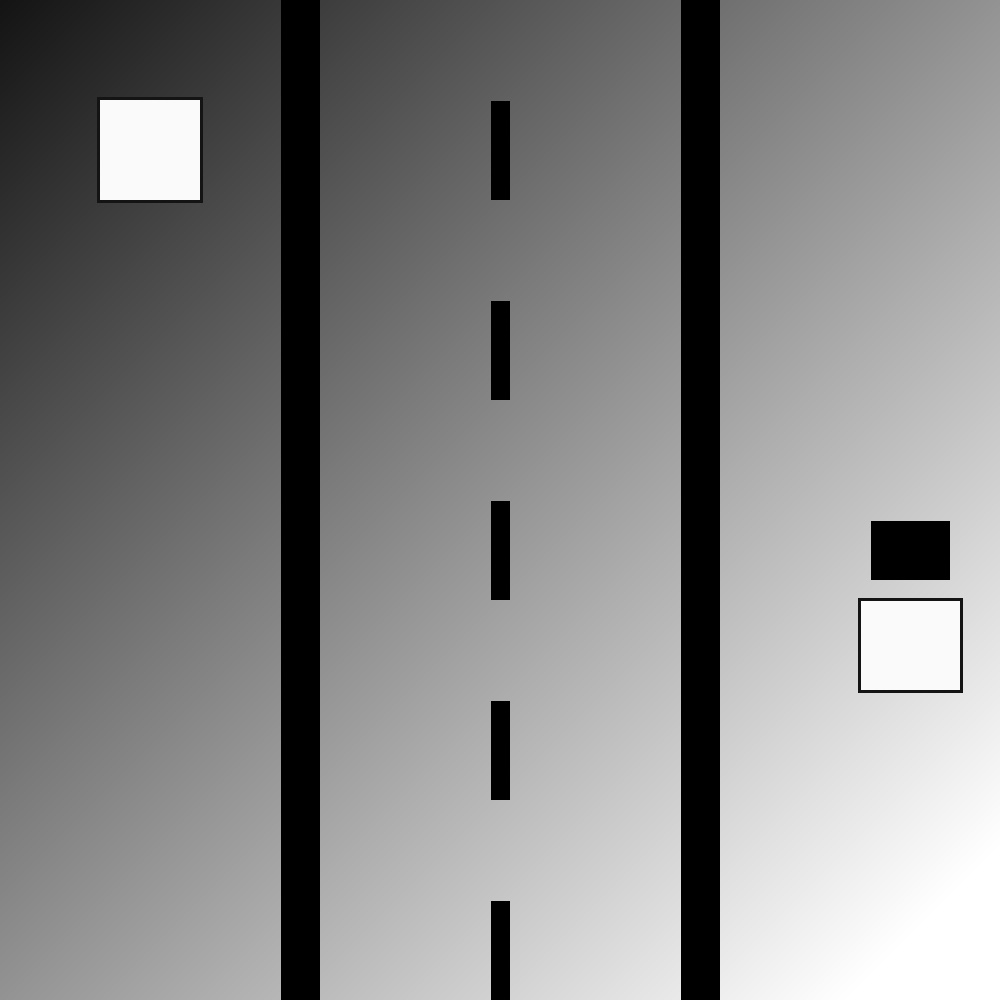
\includegraphics[height=3in]{flat_image.jpg}}
\subfloat[DEM Information]{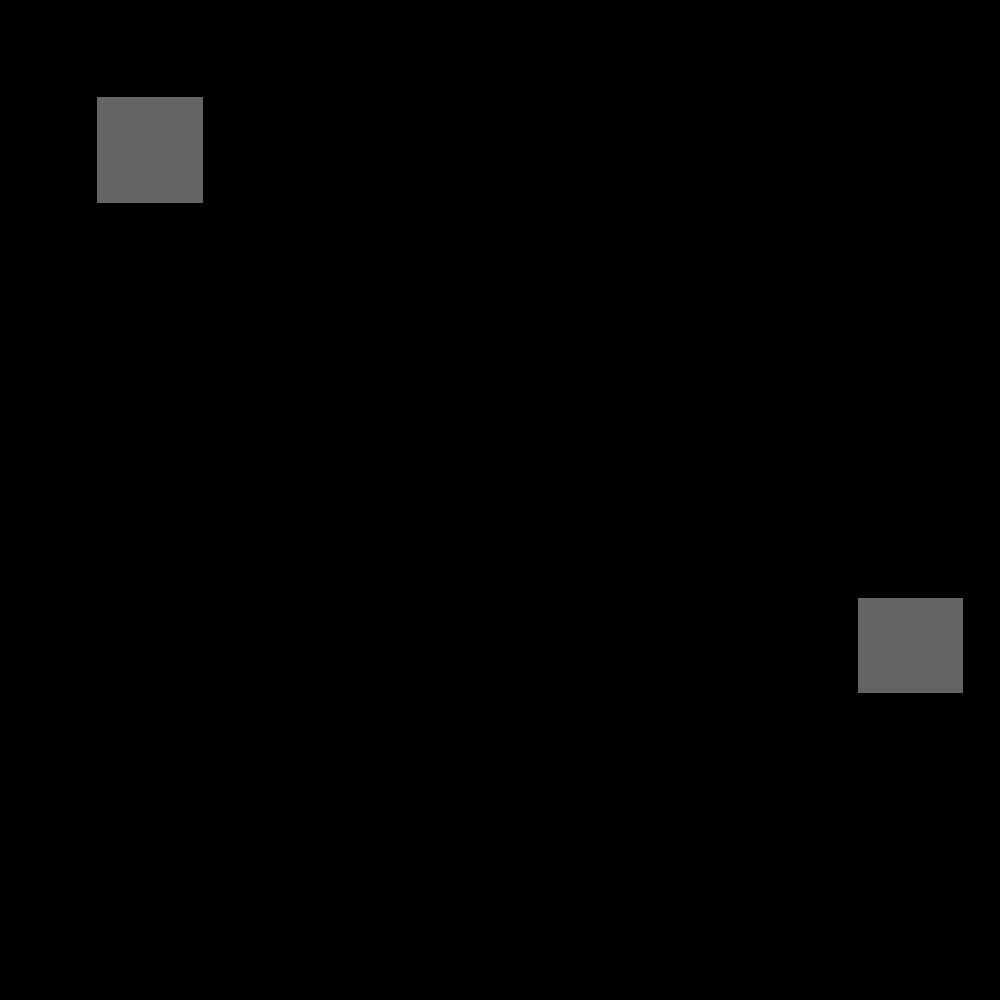
\includegraphics[height=3in]{dem.png}}
\caption{Test image generated prior to rotation.  The dem ranges from 0 to 100 meters. The test image is 1K by 1K.}
\end{figure}


%%%%%%%%%%%%%%%%%%%%%%%%%%%%%%%%%%%%%%%%%%%%%%
%                   TEST 1                   %
%%%%%%%%%%%%%%%%%%%%%%%%%%%%%%%%%%%%%%%%%%%%%%
\clearpage
\section*{Test 1}

%%%  RUN CHARACTERISTICS %%%%
\begin{itemize}
\item[] Rotation angle: 0
\item[] Rotation axis: $(1,0,0)$
\end{itemize}

%%%% WITHOUT PERSPECTIVE %%%%%%%
\begin{figure}[!h]
\centering
\subfloat[Without Perspective        ]{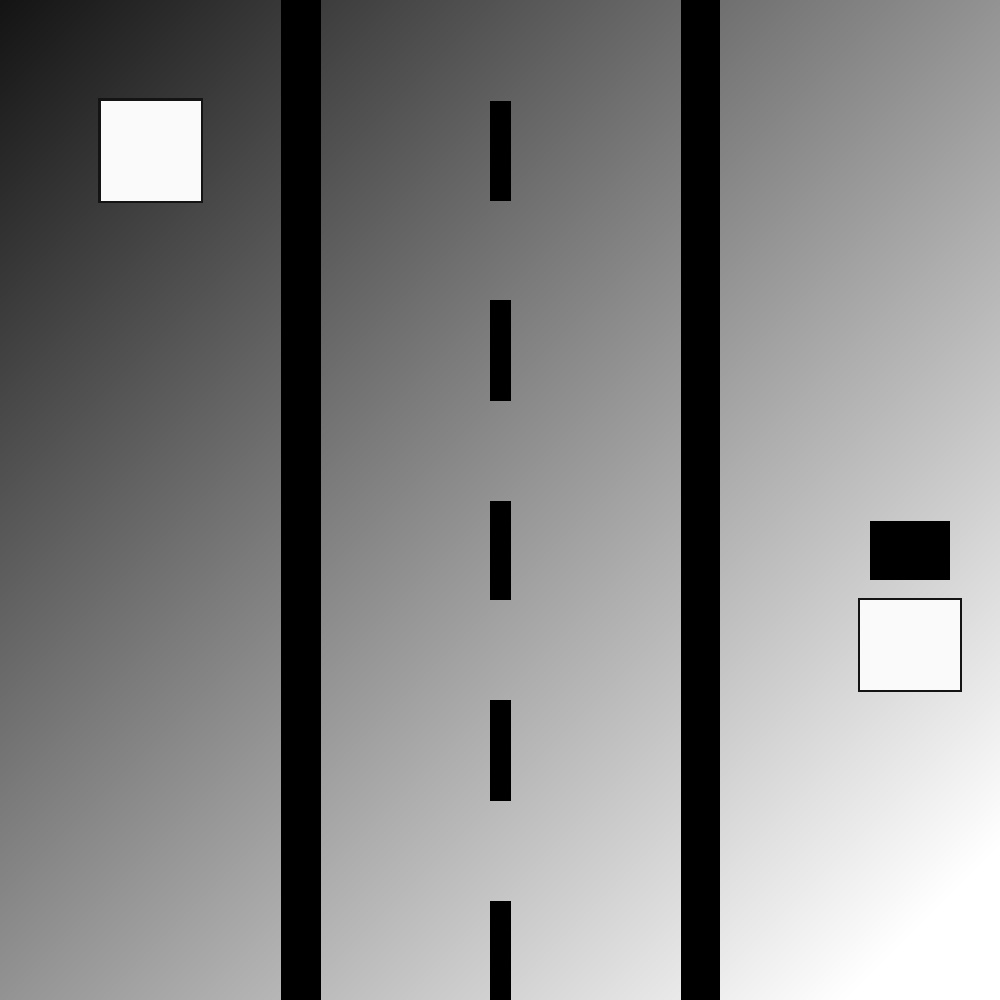
\includegraphics[height=2.0in]{test1_no_perspective.jpg}}
\hspace{1mm}
\subfloat[With Perspective           ]{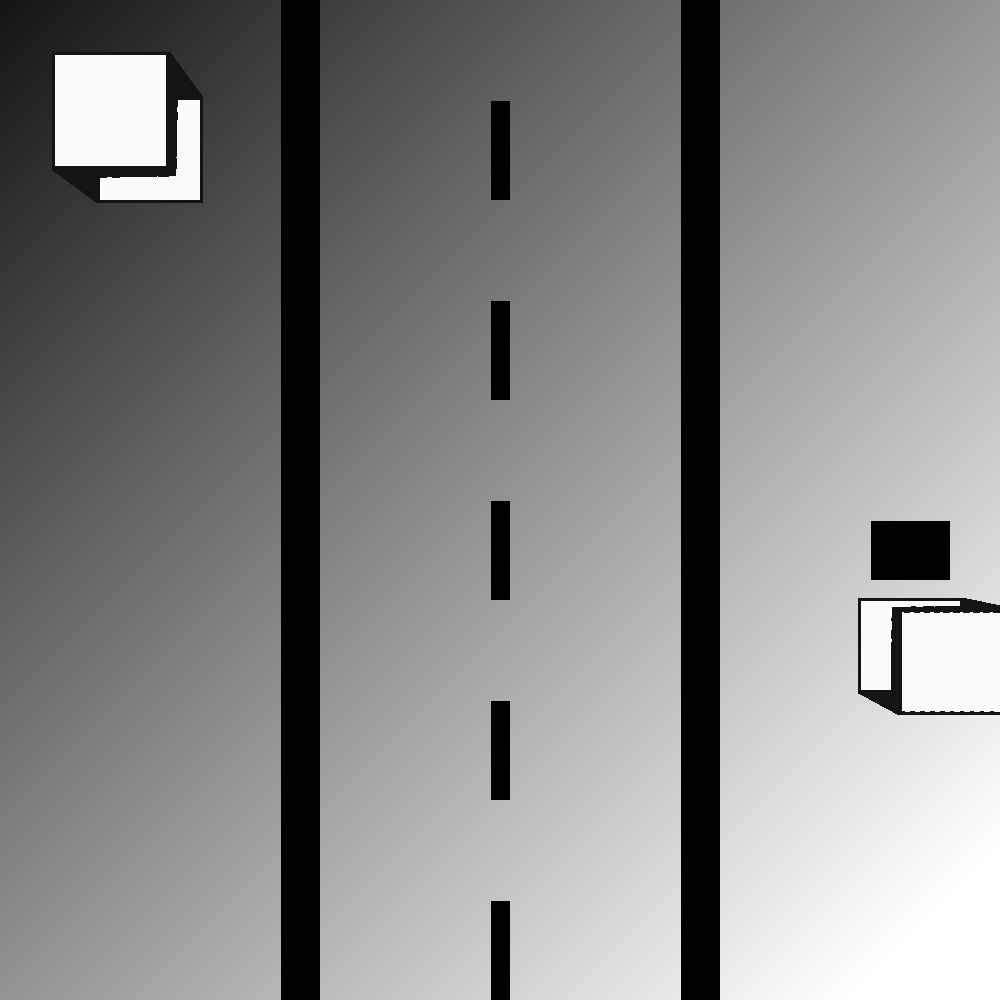
\includegraphics[height=2.0in]{test1_perspective.jpg}}\\
%%%  WITH PERSPECTIVE %%%%%
\subfloat[Rectified w/out Perspective]{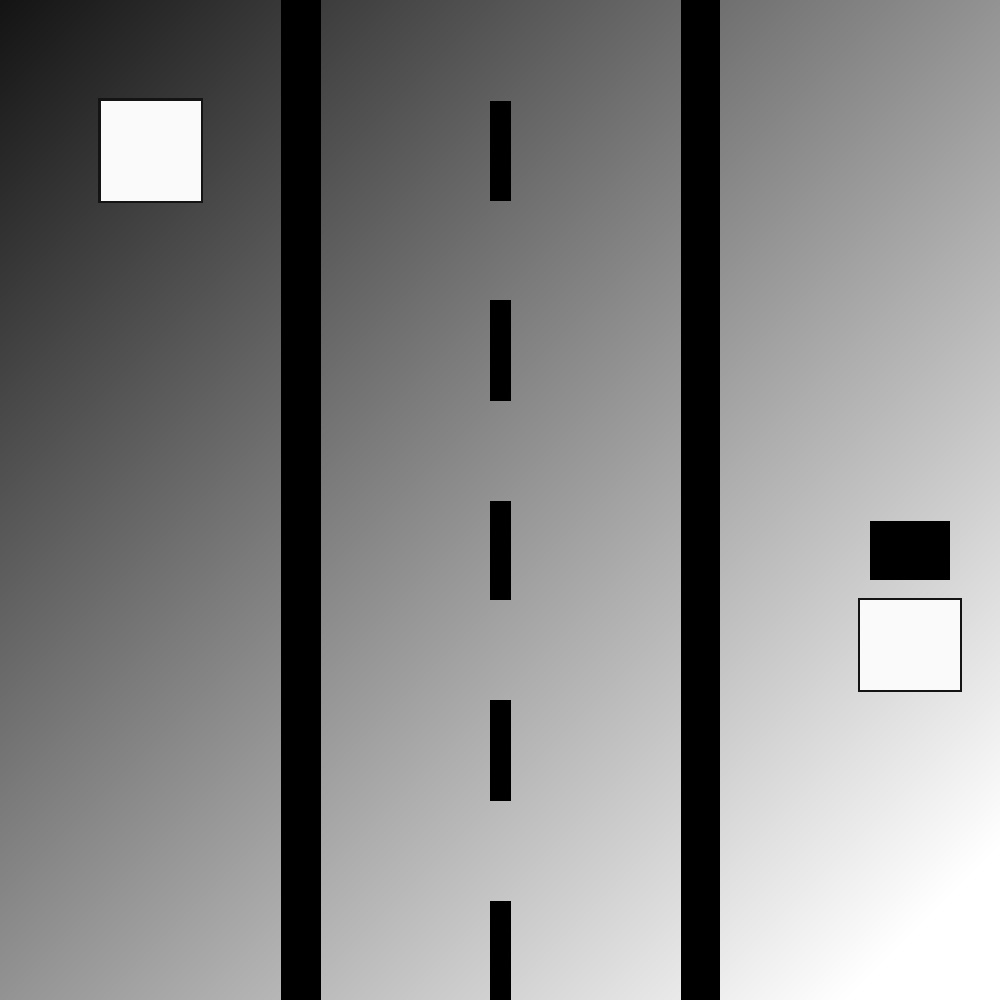
\includegraphics[height=2.0in]{test1_rectified_no_perspective.jpg}}
\hspace{1mm}
\subfloat[Rectified w/out DEM Data   ]{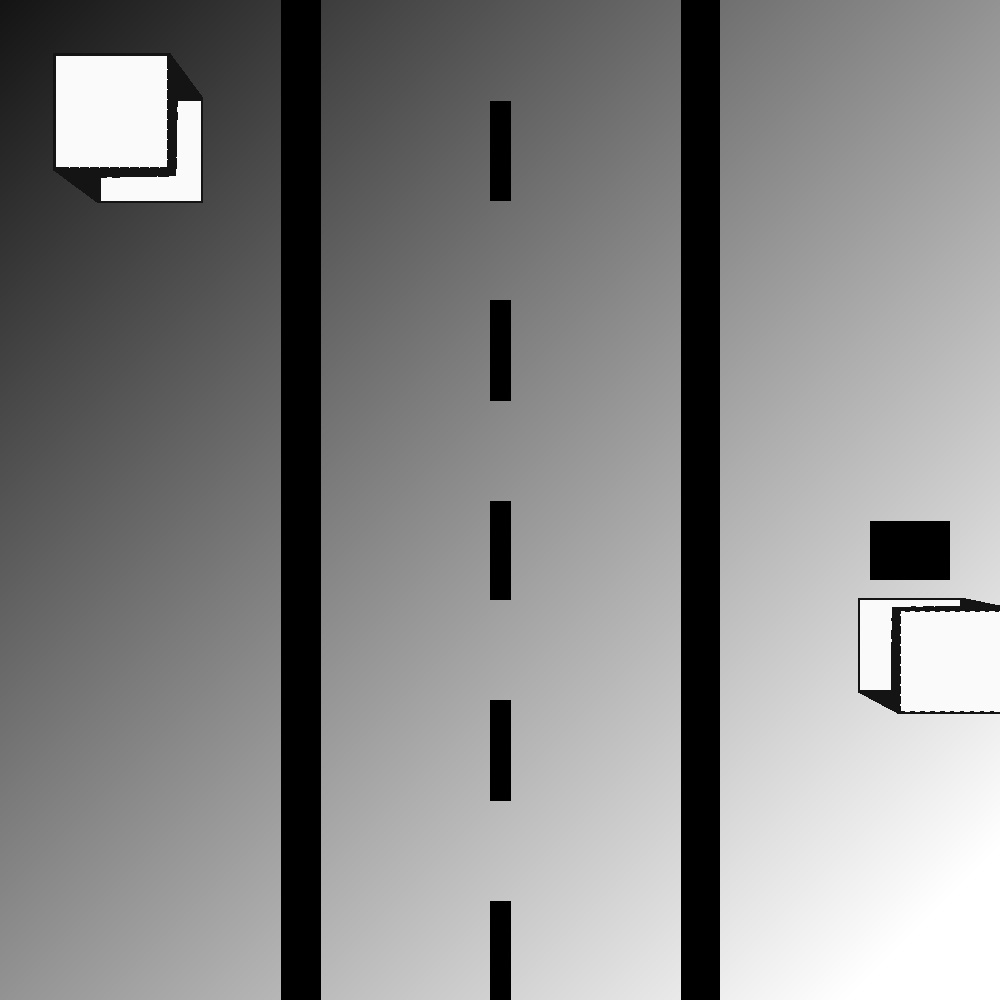
\includegraphics[height=2.0in]{test1_nodem_perspective.jpg}}
\hspace{1mm}
\subfloat[Rectified with  DEM Data   ]{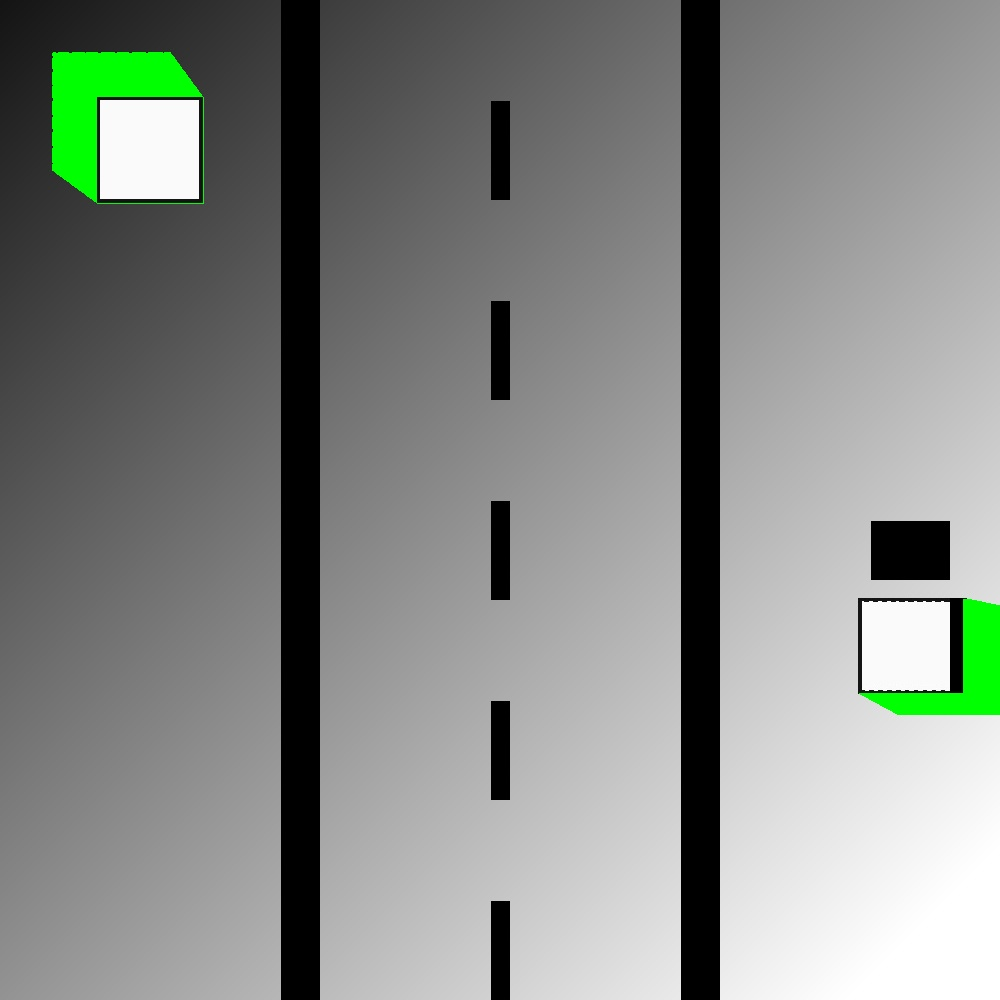
\includegraphics[height=2.0in]{test1_complete.jpg}}
\caption{Results from test.  Note that the green represents invalid regions where the point
         was occluded. Most of the images look alike, as there is no rotation, just a conversion
         from perspective projection into parallel projection.}
\end{figure}


%%%%%%%%%%%%%%%%%%%%%%%%%%%%%%%%%%%%%%%%%%%%%%
%                   TEST 2                   %
%%%%%%%%%%%%%%%%%%%%%%%%%%%%%%%%%%%%%%%%%%%%%%
\clearpage
\section*{Test 2}

%%%  RUN CHARACTERISTICS %%%%
\begin{itemize}
\item[] Rotation angle: 45
\item[] Rotation axis: $(1,0,0)$
\end{itemize}

%%%% WITHOUT PERSPECTIVE %%%%%%%
\begin{figure}[!h]
\centering
\subfloat[Without Perspective        ]{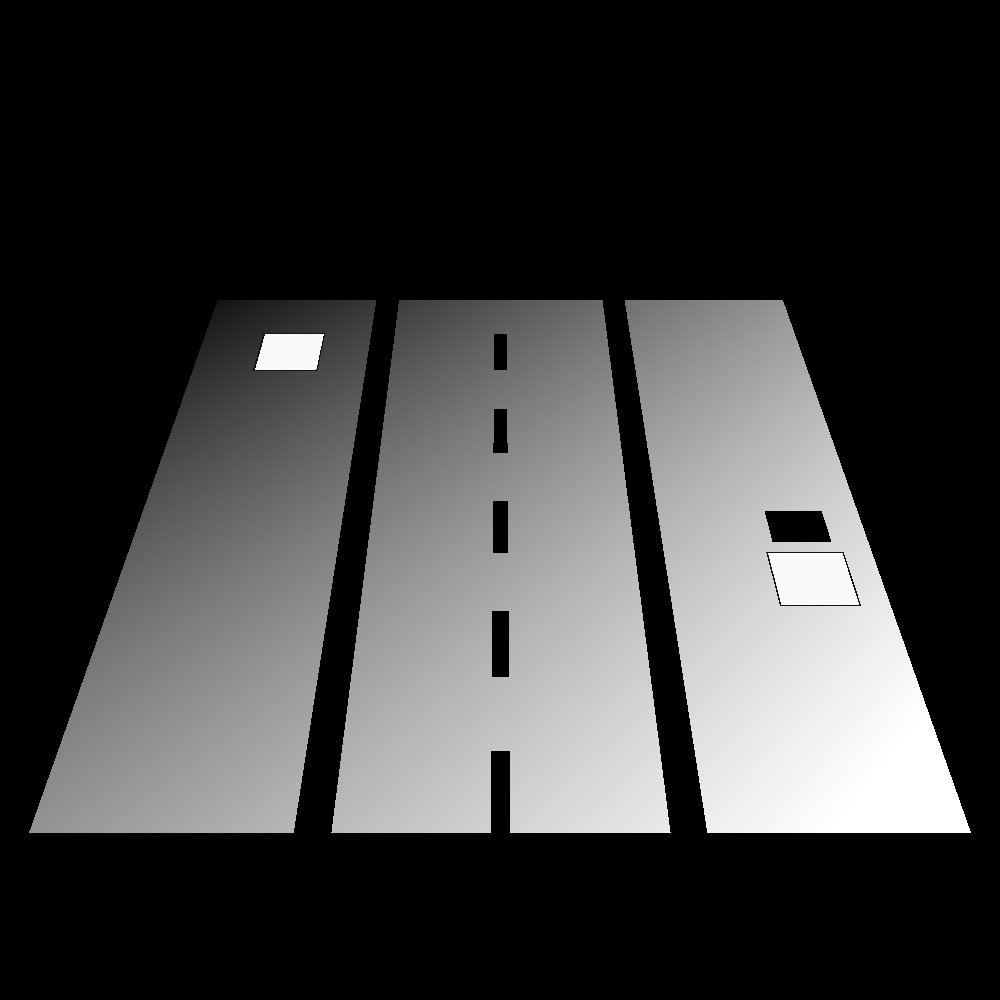
\includegraphics[height=3.0in]{test2_no_perspective.jpg}}
\hspace{1mm}
\subfloat[Rectified                  ]{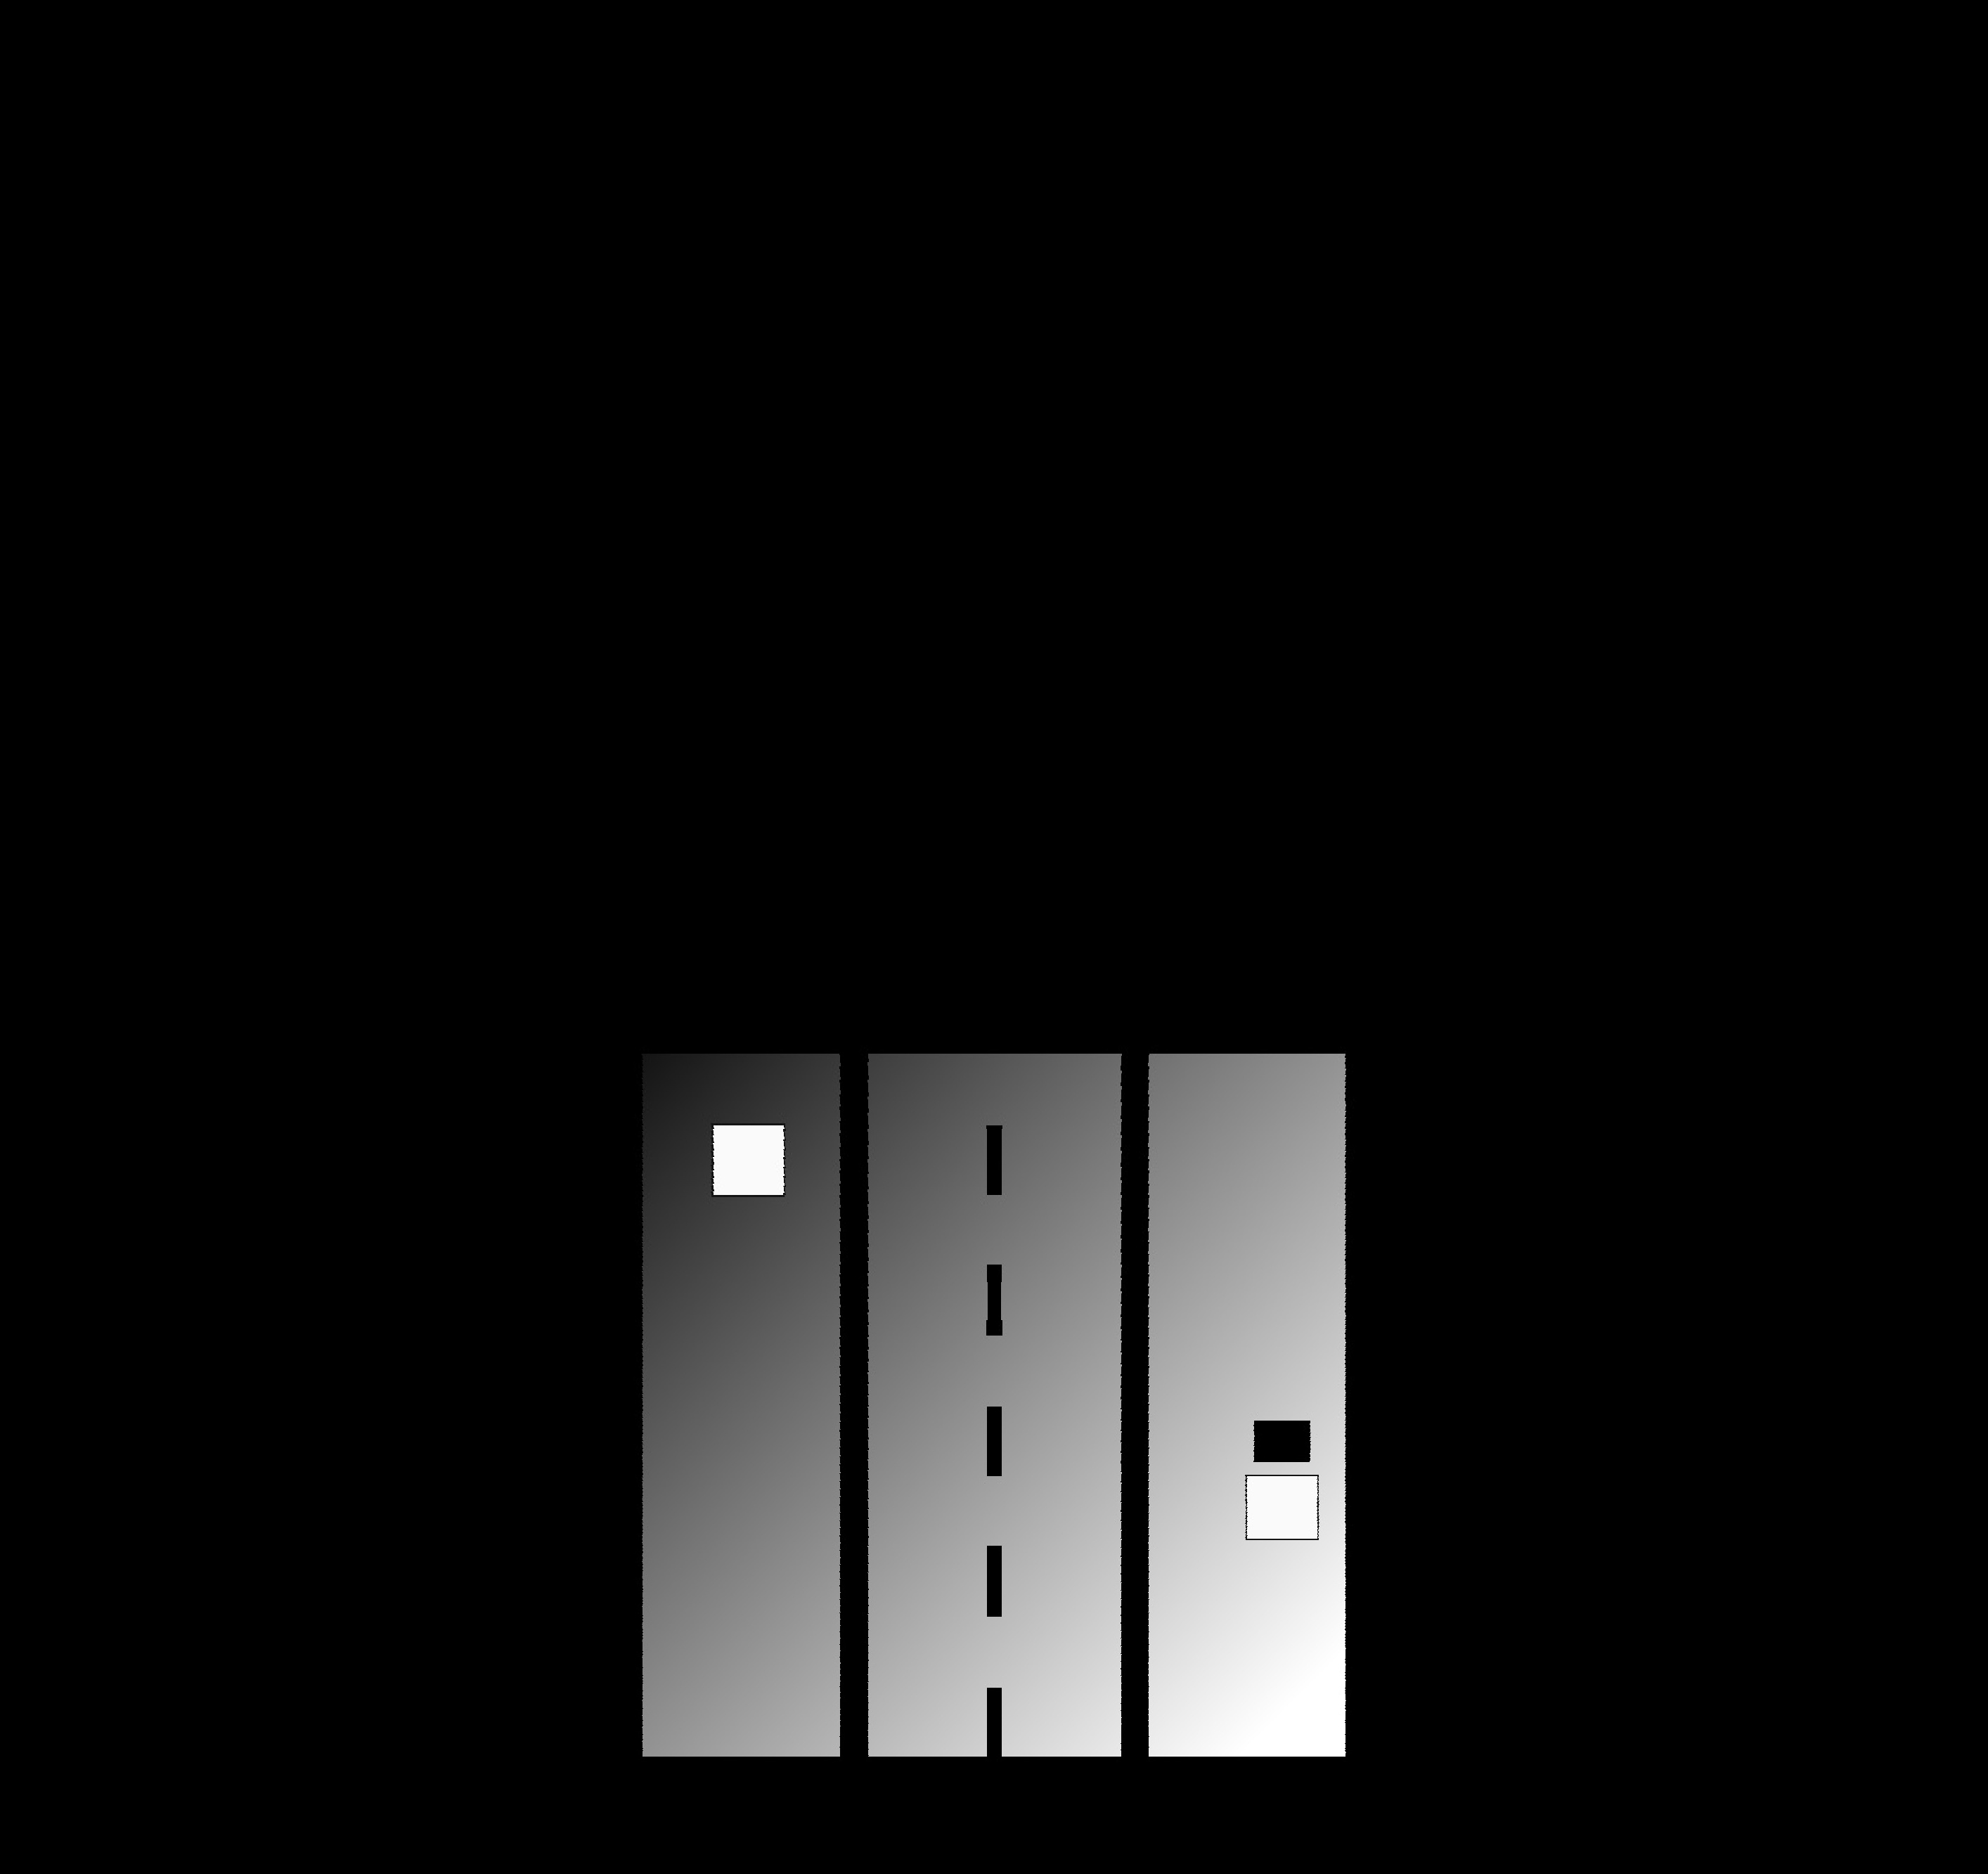
\includegraphics[height=3.0in]{test2_rectified_no_perspective.jpg}}\\
\caption{The rectified box is actually the same size as the original image. The rectified image is just much, much larger. 
         This is due to the corners of the full "earth plane" extending past the box.  If this
         was a geographic image and contained full information as not shown in the image without perspective, the tails of
         this image would be severly stretched.}
\end{figure}

\begin{figure}[!h]
\centering
%%%  WITH PERSPECTIVE %%%%%
\subfloat[With Perspective           ]{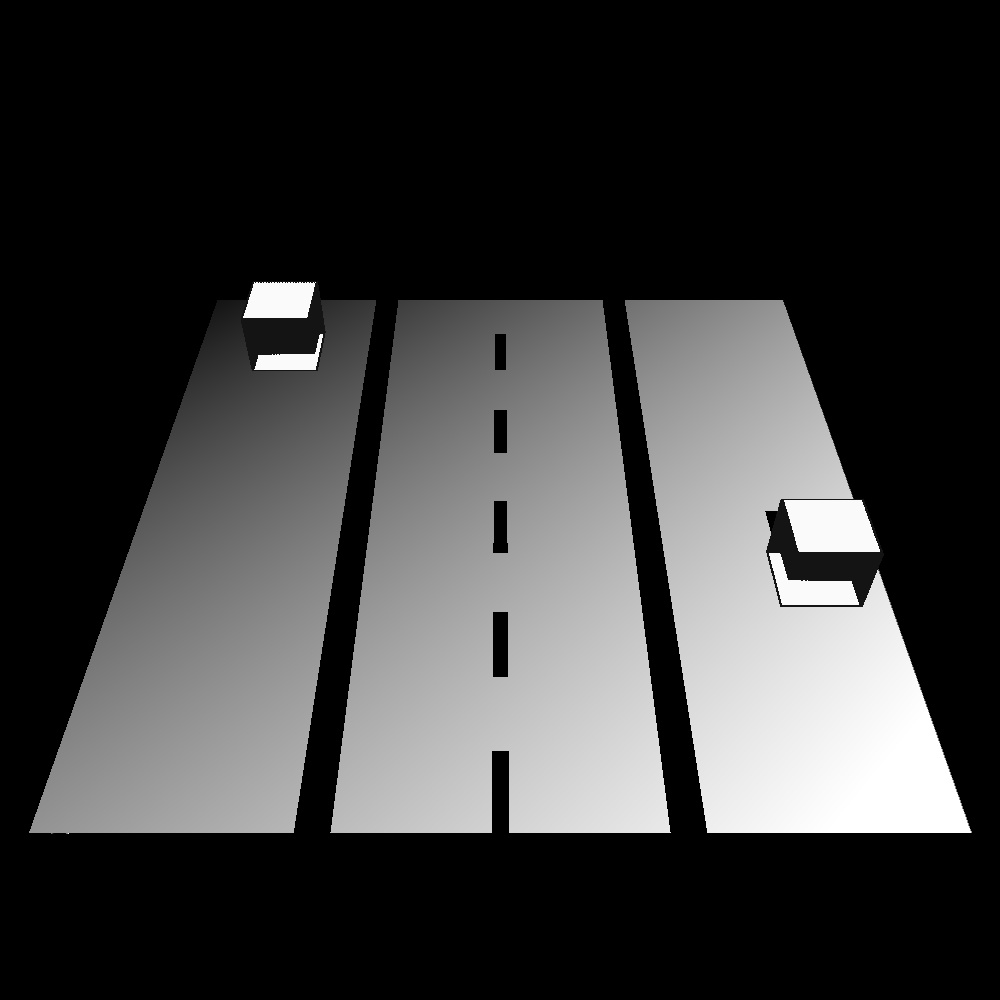
\includegraphics[height=3.0in]{test2_perspective.jpg}}\\
\subfloat[Rectified w/out DEM Data   ]{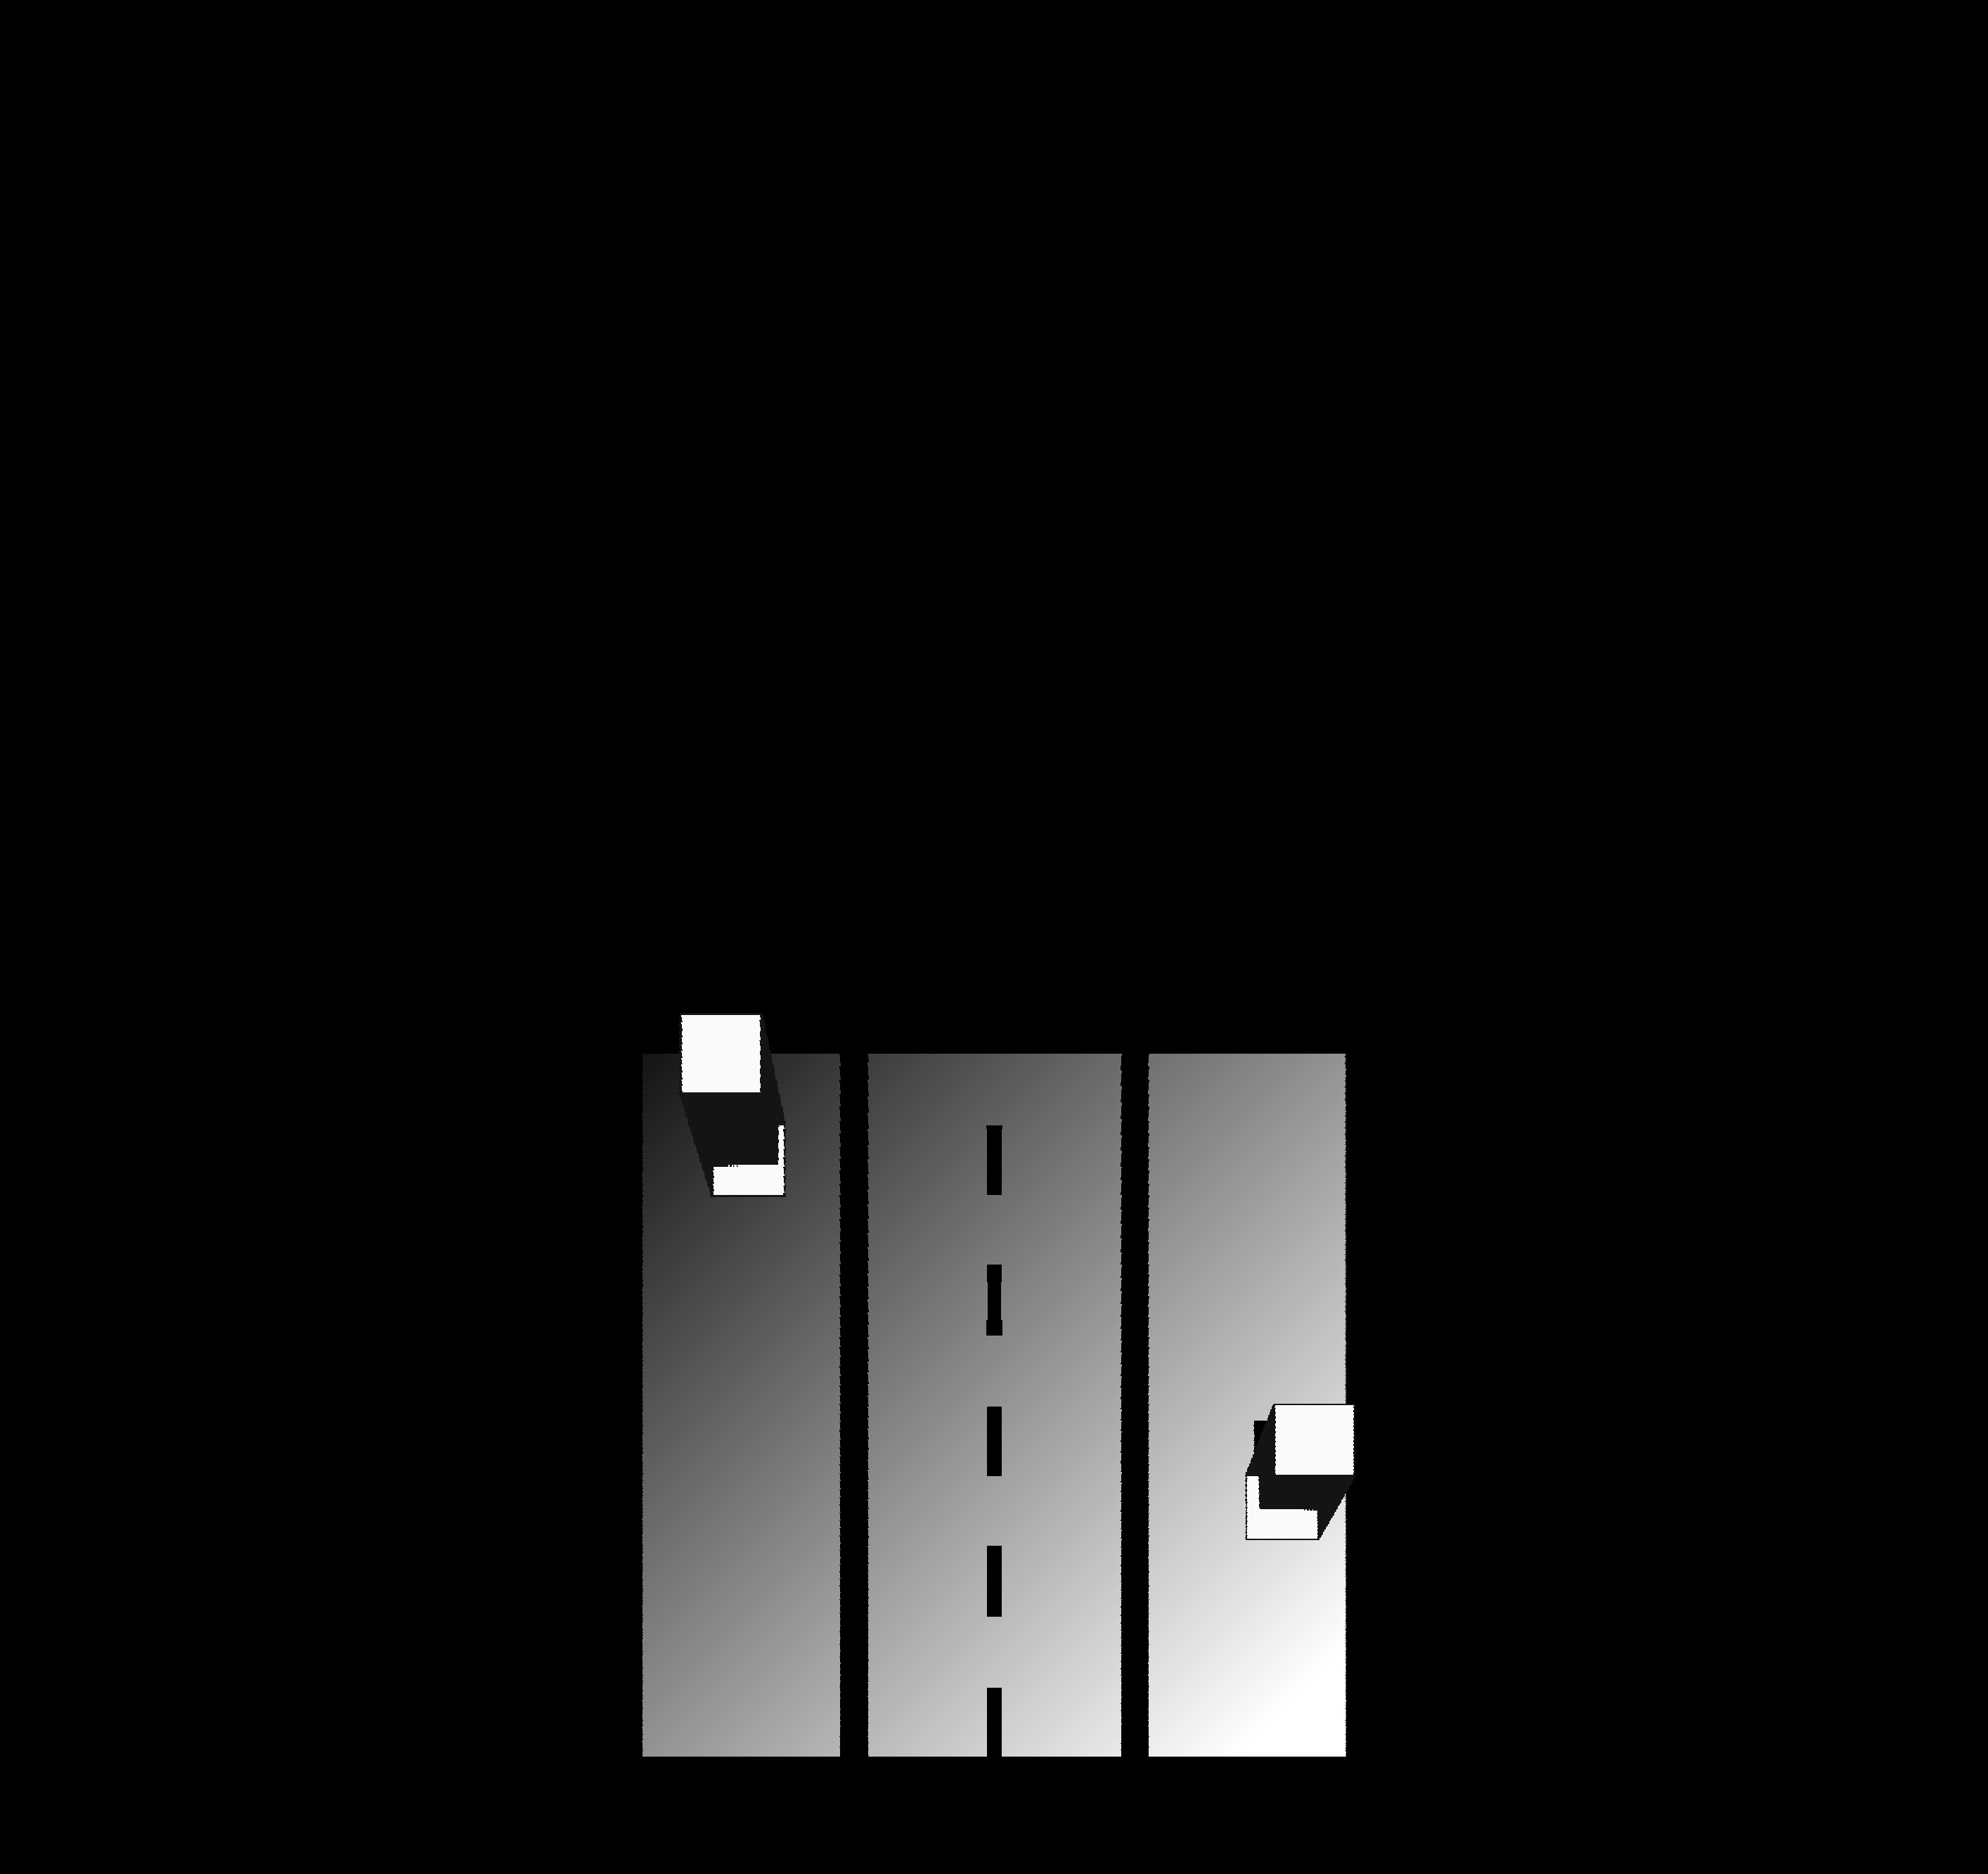
\includegraphics[height=3.1in]{test2_nodem_perspective.jpg}}
\subfloat[Rectified with  DEM Data   ]{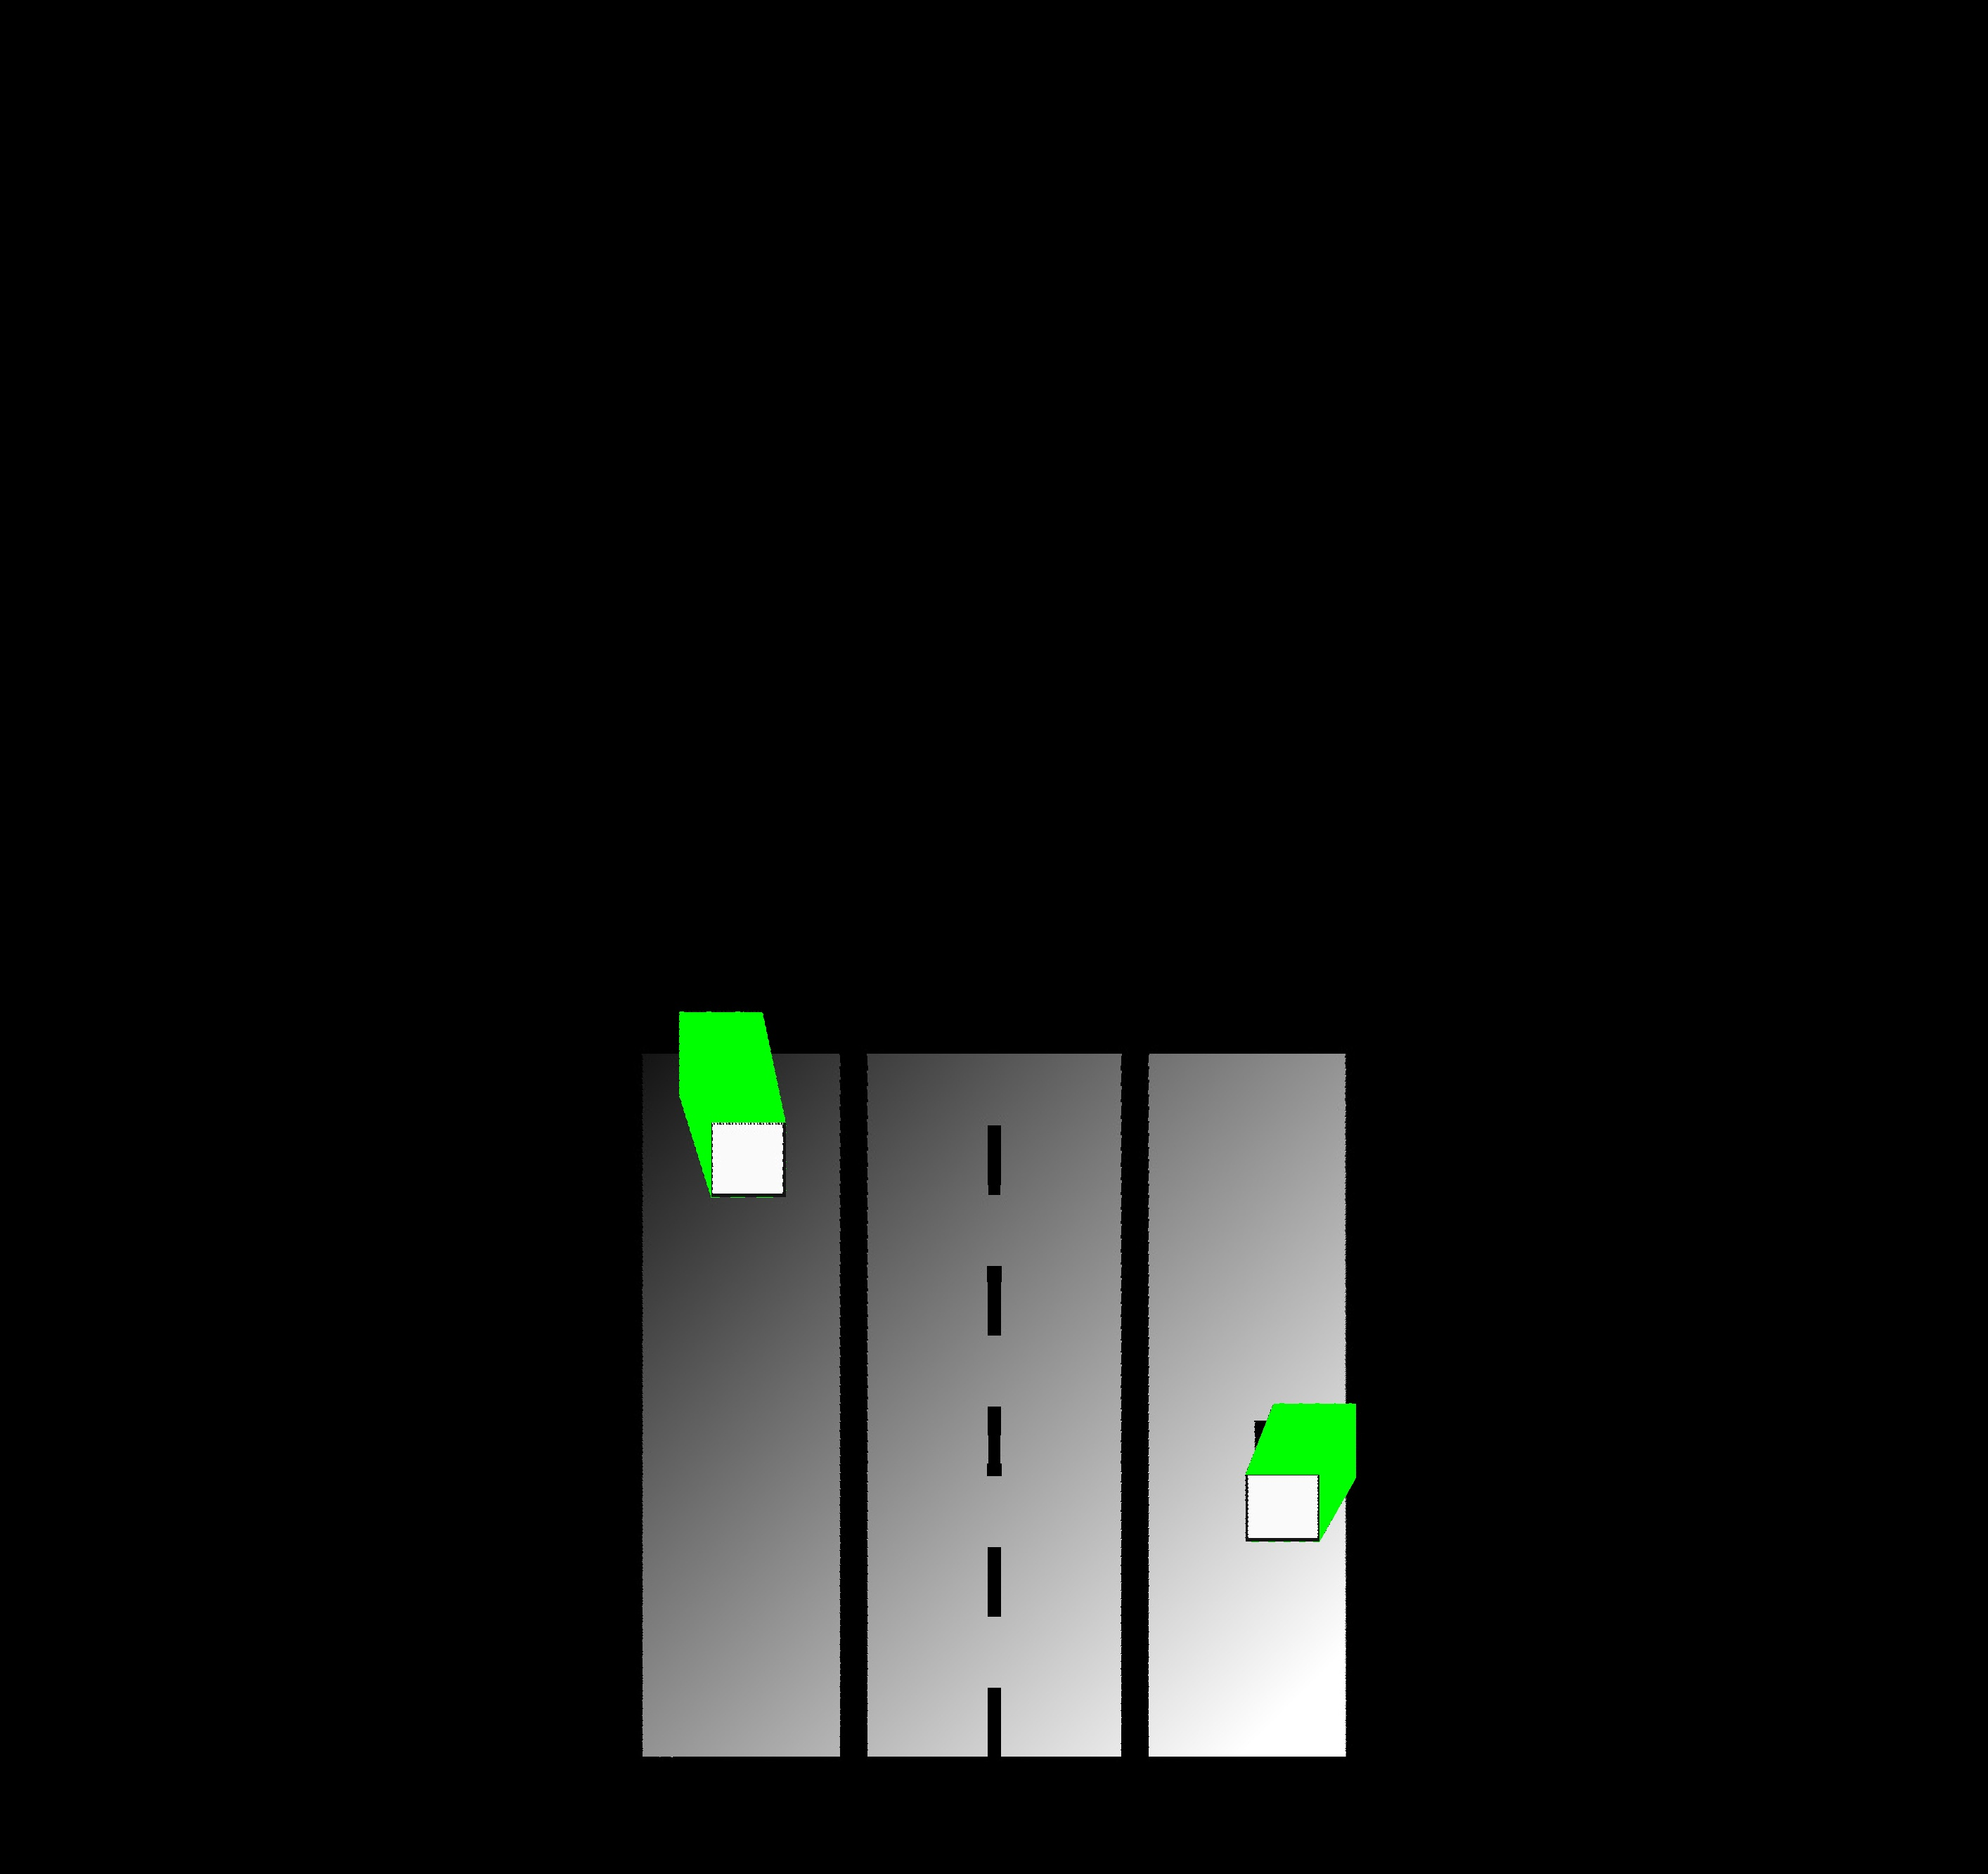
\includegraphics[height=3.1in]{test2_complete.jpg}}
\caption{Results from test.  Note that the green represents invalid regions where the point
         was occluded.}
\end{figure}

%%%%%%%%%%%%%%%%%%%%%%%%%%%%%%%%%%%%%%%%%%%%%%
%                   TEST 3                   %
%%%%%%%%%%%%%%%%%%%%%%%%%%%%%%%%%%%%%%%%%%%%%%
\clearpage
\section*{Test 3}

%%%  RUN CHARACTERISTICS %%%%
\begin{itemize}
\item[] Rotation angle: 45
\item[] Rotation axis: $(1,1,1)$
\end{itemize}

%%%% WITHOUT PERSPECTIVE %%%%%%%
\begin{figure}[!h]
\centering
\subfloat[Without Perspective        ]{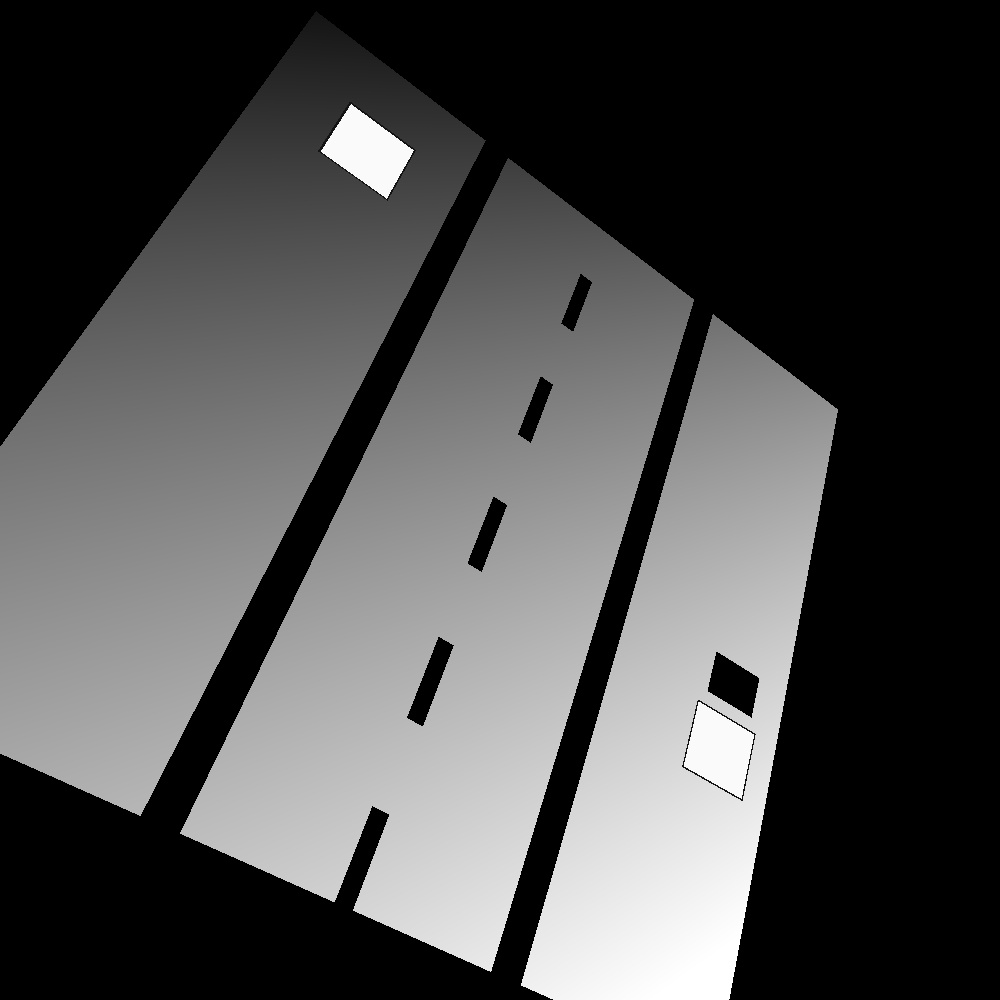
\includegraphics[height=3.0in]{test3_no_perspective.jpg}}
\hspace{1mm}
\subfloat[Rectified                  ]{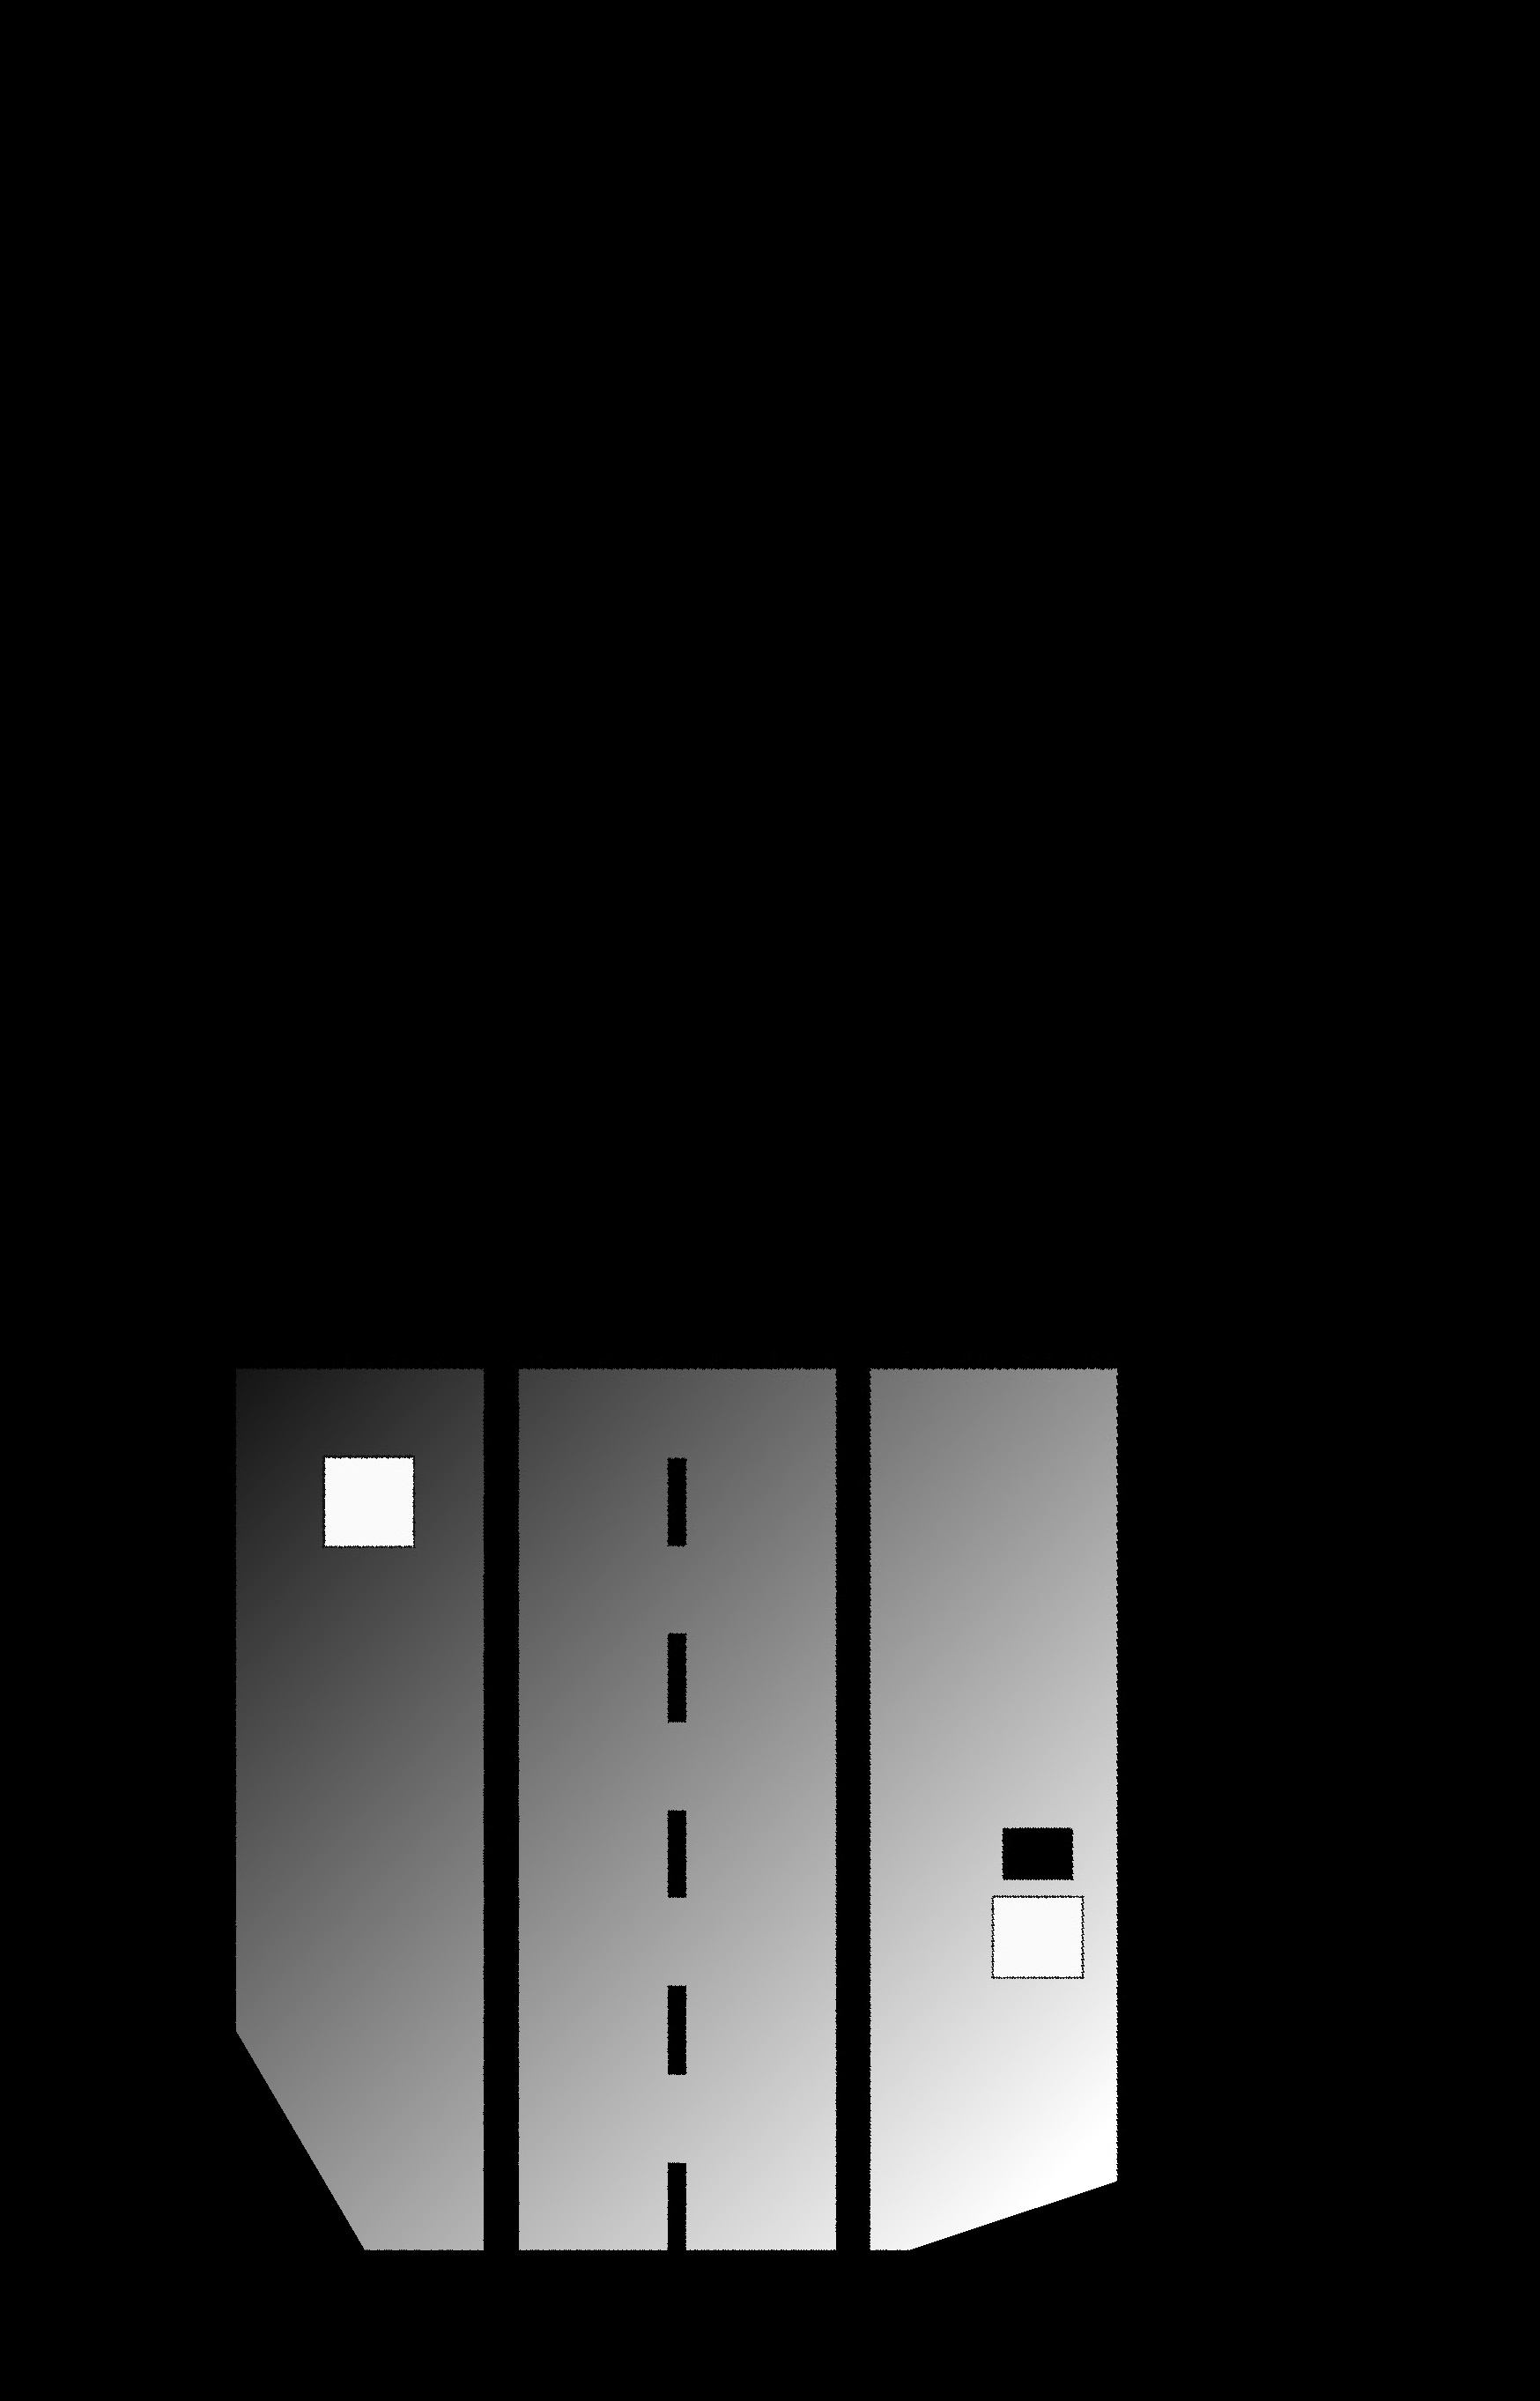
\includegraphics[height=3.0in]{test3_rectified_no_perspective.jpg}}\\
\end{figure}

\begin{figure}[!h]
\centering
%%%  WITH PERSPECTIVE %%%%%
\subfloat[With Perspective           ]{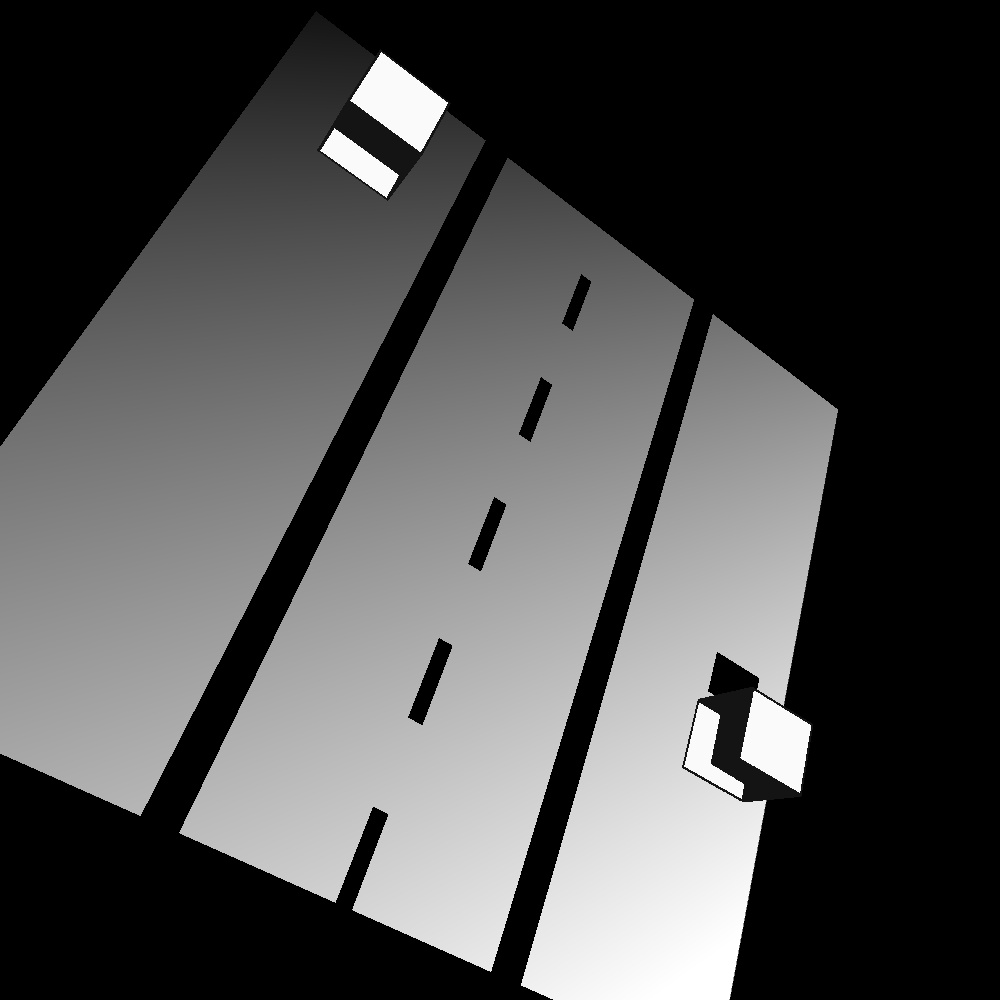
\includegraphics[height=3.0in]{test3_perspective.jpg}}\\
\subfloat[Rectified w/out DEM Data   ]{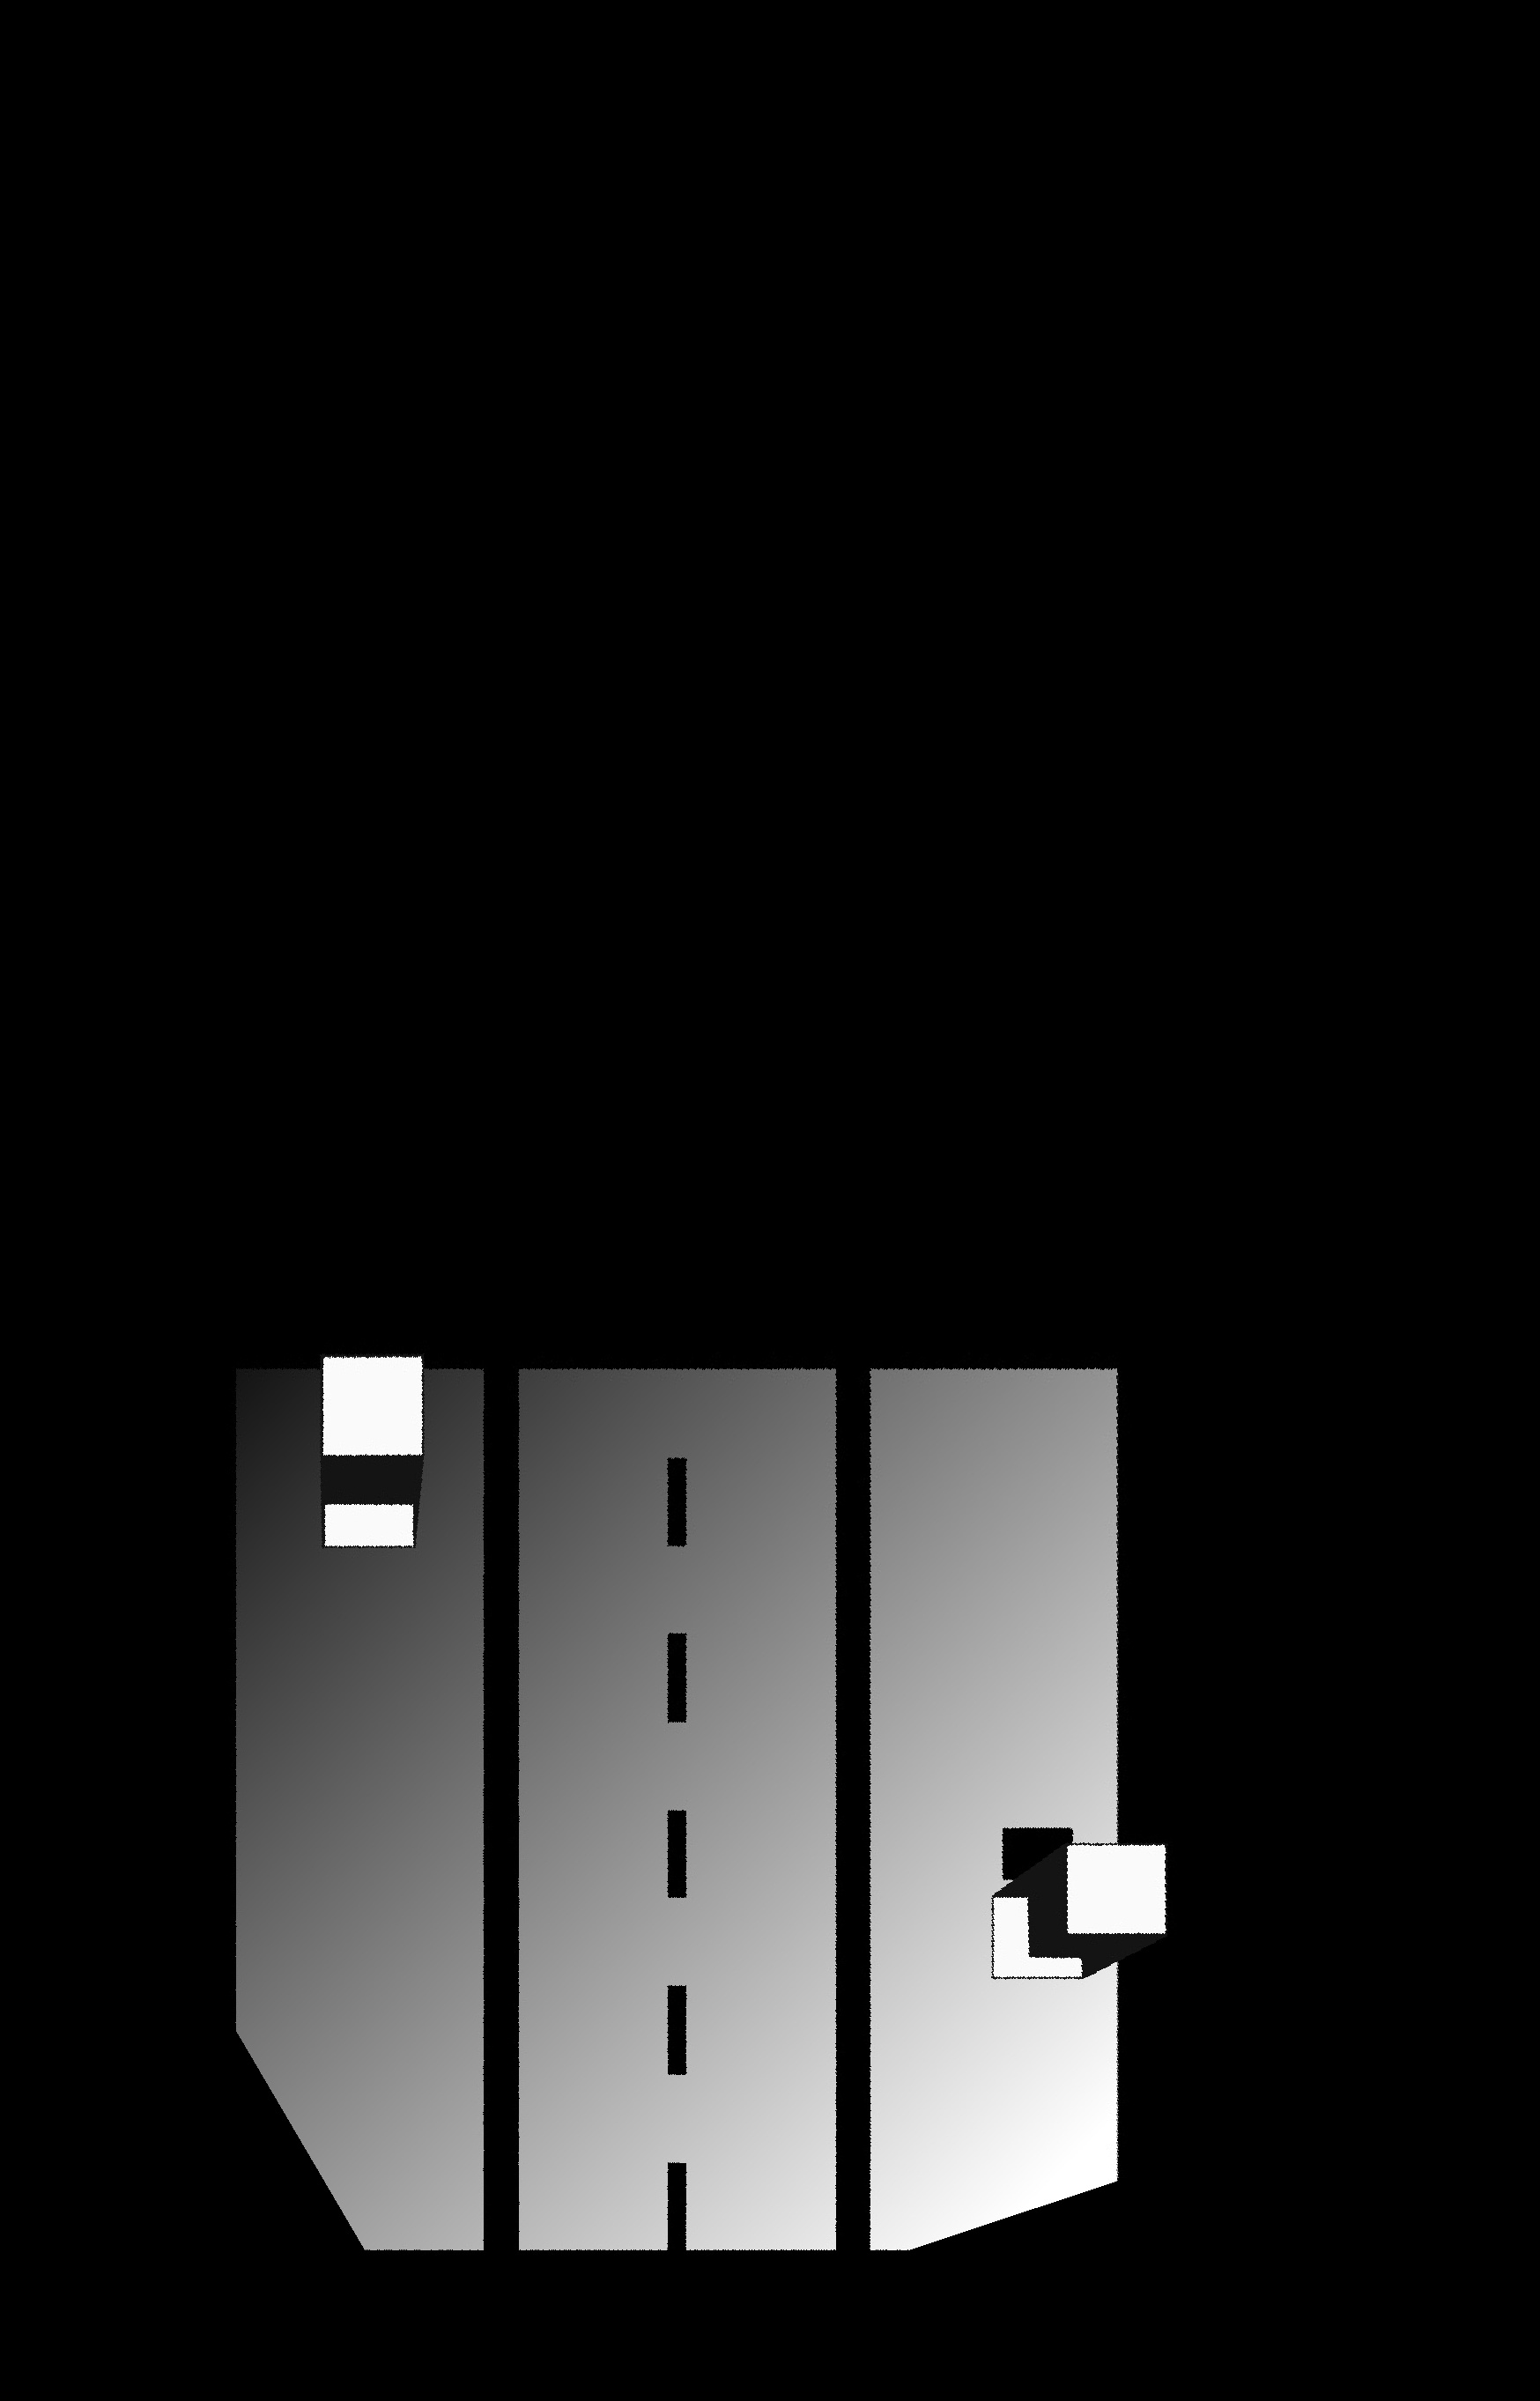
\includegraphics[height=4.1in]{test3_nodem_perspective.jpg}}
%\subfloat[Rectified with  DEM Data   ]{\includegraphics[height=4.1in]{test3_complete.jpg}}
\caption{Results from test.  Note that the green represents invalid regions where the point
         was occluded.}
\end{figure}


\end{document}
